  \begin{appendices}

\chapter{First appendix}
  \section{IP Header Struct}
  Let us now look at the actual \textbf{iphdr struct:} \\
  
\begin{lstlisting}
struct iphdr {
 #if defined(__LITTLE_ENDIAN_BITFIELD)
     __u8    ihl:4,
                 version:4;
 #elif defined (__BIG_ENDIAN_BITFIELD)
      __u8    version:4,
              ihl:4;
 #else
 #error  "Please fix <asm/byteorder.h>"
 #endif
       __u8    tos;
       __u16   tot_len;
       __u16   id;
       __u16   frag_off;
       __u8    ttl;
       __u8    protocol;
       __u16   check;
       __u32   saddr;
       __u32   daddr;
        /*The options start here. */
};
\end{lstlisting} 

The struct uses the correct version number, which alternates between big endian and little endian depending on the machines architectural set up. (Note: This thesis assumes the concept  of little endian, big endian is known to the reader. If not, be aware that it is not crucial to the understanding of the thesis). 


  \section{TCPhdr Struct}

\begin{lstlisting}
 struct tcphdr {
         __u16   source;
         __u16   dest;
         __u32   seq;
         __u32   ack_seq;
 #if defined(__LITTLE_ENDIAN_BITFIELD)
         __u16   res1:4,
                 doff:4,
                 fin:1,
                 syn:1,
                 rst:1,
                 psh:1,
                 ack:1,
                 urg:1,
                 ece:1,
                 cwr:1;
 #elif defined(__BIG_ENDIAN_BITFIELD)
         __u16   doff:4,
                 res1:4,
                 cwr:1,
                 ece:1,
                 urg:1,
                 ack:1,
                 psh:1,
                 rst:1,
                 syn:1,
                 fin:1;
 #else
 #error  "Adjust your <asm/byteorder.h> defines"
 #endif  
        __u16   window;
        __u16   check;
        __u16   urg_ptr;
};
\end{lstlisting}


\subsection*{Brief recap of Binary Search Tree(BST)}
The Binary Search Tree(BST) data structure will provides an efficient way to store, search and retrieve data (IP to MAC address mappings in our case). As can be seen in the data struct node, we have a node struct that contains two other node structs pointers called "left" and "right". This "node within a node" recursive structure will give us a recursive algorithm which allows for searching time of O(h) worst case runtime complexity where h stands for the height of the tree. As can be seen in Fig 4.12, a BST structure has has at least O(log n) levels for n number of nodes. It will thus make O(log n) comparisons at a minimum to find a target node. This is ideal in terms of both speed and CPU efficiency, since we will be perusing through multiple ip addresses per second on the satellite link. 

\begin{figure}[h!]
	\centering
    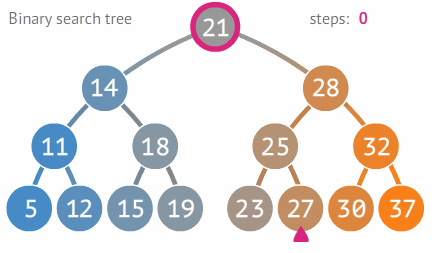
\includegraphics[width=0.87\textwidth]{BST.PNG}
    \caption{BST Structure}
    \label{fig:BST}
\end{figure}

In a standard BST structure the nodes are ordered as follows:

\begin{itemize}
\item each node contains one key (or data-in our case, our struct nodes key is "IP address" and its corresponding "MAC address" mapping is the nodes data).
\item the keys for a nodes left subtree are smaller than the key in its parent node.;
\item the keys for a nodes right subtree are bigger than the key in its parent node.;
\item Cannot have the same key in different nodes of the tree.\\
\end{itemize}

The writers assumption here is that Binary Search Tree algorithm is standard knowledge for the reader (if not, see section 2.3.4 "Topics to review"). Our PEP code incorporates the use of this BST structure to build our ARP Table cache. \\

\section{Challenges encountered}

Many unforeseen challenges encountered while creating the PEP coupled with the one year time constraints of a Masters thesis paper, hindered our ability to deliver a complete final product. In short, we did not have enough time to implement all of the proposed PEP logic planned for the PEP. The receiver window size (rwnd) as described previously in chapter 2 \emph{TCP flow control} was initially going to be a crucial part of our PEP. One of our aims for this project was to create a PEP where we could dynamically alter the receiver window size to adjust for congestion and idleness on the degraded bottleneck satellite link. This facet of the PEP, however, will be implemented as future work to improve the performance of the PEP. More detail will be provided in the next chapter on how this will work with our current PEP implementation.

\subsection{Kernel overriding code interface commands}
One problem that had not been anticipated was the kernel overriding code interface commands. We had coded our packets to be forwarded out a specific interface on our PEP via raw socket programming commands. The kernel, however, was calculating the best path and forwarding the packet out the interface it deemed best to suit that path. The interface chosen by the kernel was not always the one we had selected as the packets exit point (but quite often it was which aided the confusion), so it took some lengthy debugging time before being able to isolate the cause of the problem. A complete overhaul of the code was needed as we realised we would need to use struct sockaddr\textunderscore ll (see Appendix B) \todo{promise} for portions of our code, where it had not been previously, to reach into data link layer to override the kernel. 
In most socket programming applications, one can leave the assembly of Ethernet and IP header to the kernel. In raw socket programming, we can leave the assembly of Ethernet, as well as ARP requests for next-hop forwarding to the kernel. In our case, however, we need to spoof ACKs - and this means using a sender IP address that is not that of the interface we are sending from. This necessitates the use of sockaddr\textunderscore ll. 

\subsection{Creating own ARP requests and ARP tables for next hop forwarding}
Another issue involved having to create our own ARP table, and ARP requests to enable us to retrieve the destination MAC address for packets we wanted to forward (up until this point, our code had been hardcoding the destination Mac address to make our testing smoother). This required code that could assemble (and then send) an ARP request packet based on the IP address we receive from the sniffer and read the ARP reply we get back from the relevant target host to whom the IP address belonged. This task involved the use of our own customised binary search tree ARP cache table for our PEP to store a record of IP address to MAC mappings found.  \\

Alternatively, rather than handling the address resolution ourselves, we could have chosen to use a call to the popen() function, which we could have used to execute the ARP command and then parse its output. The problem, however, is that the \emph{popen()} function starts a new separate process and we could be calling this function quite often depending on the size of the local subnet that the PEP is directly connected to and the number of active hosts in that subnet we would have needed to resolve. Opening multiple additional processes in a time-critical environment, such as our PEP, would have adverse effects on performance, so the \emph{popen()} option was abandoned. \\

\subsection{Fine tuning ARP responses via non-blocking sockets}

Late into the coding process, we inadvertently discovered that we had what turned out to be a significant problem in that we were using the incorrect type of sockets. We stumbled upon this discovery while trying to fine tune our reception of ARP responses. Our current code would send out an ARP request on the forward interface, and our PEP would listen for the corresponding ARP response. If for instance, however, we never get an ARP response because the IP is local, but there is no such host on the network, the {\tt recv()} socket function will automatically \emph{block}. In other words, the {\tt recv()} function will not return until it has received a packet. Since there is no packet coming, the PEP will wait forever and stall. During this time, none of the other code executes, so we can not receive packets on the incoming interface, or perform any other actions in the PEP. The solution was to have a look at non-blocking sockets. Up until this point, we had used the standard raw sockets programming which blocks by default, so this required another code overhaul. \\

In short, non-blocking sockets does as its name suggests. They are sockets that do not block, so when we call {\tt recv()} or any other send or receive function and pass the socket as a parameter, that function will always return whether it receives a packet or not. The positive here is that this means the absence of packets will not cause our PEP to freeze, but the negative side is that it requires more code to check whether the {\tt recv()} function actually received a packet or whether it returned an empty value. \\

It eventually became apparent that the non-blocking sockets were not just crucial to the correct operation of the ARPing process, but they were in fact, also the critical element to building our PEP. In theory, the PEP needs to listen on its incoming and outgoing interfaces simultaneously. In practice, this is not possible as the socket programming has limitations that only allow it to listen on one interface at a time consecutively, although it can swap between the two interfaces at such high-speed that would make it seem almost simultaneous. While we were using the standard default blocking sockets, however, we might start listening on the one interface, but the receive function would not return until we had a packet arriving there (which could take forever, literally). Meanwhile, we might miss many packets on the other interface. Non-blocking means that if there is no packet pending on an interface, the function returns anyway (but empty-handed), so we can go on to check the other interface.

\subsection{Unavailability of the Satellite Simulator}

The University of Auckland Pacific Island Satellite Simulator was being used extensively for PhD experiments, so it was not available for use with this PEP until late January. 

\begin{figure}[h!]
    \centering
    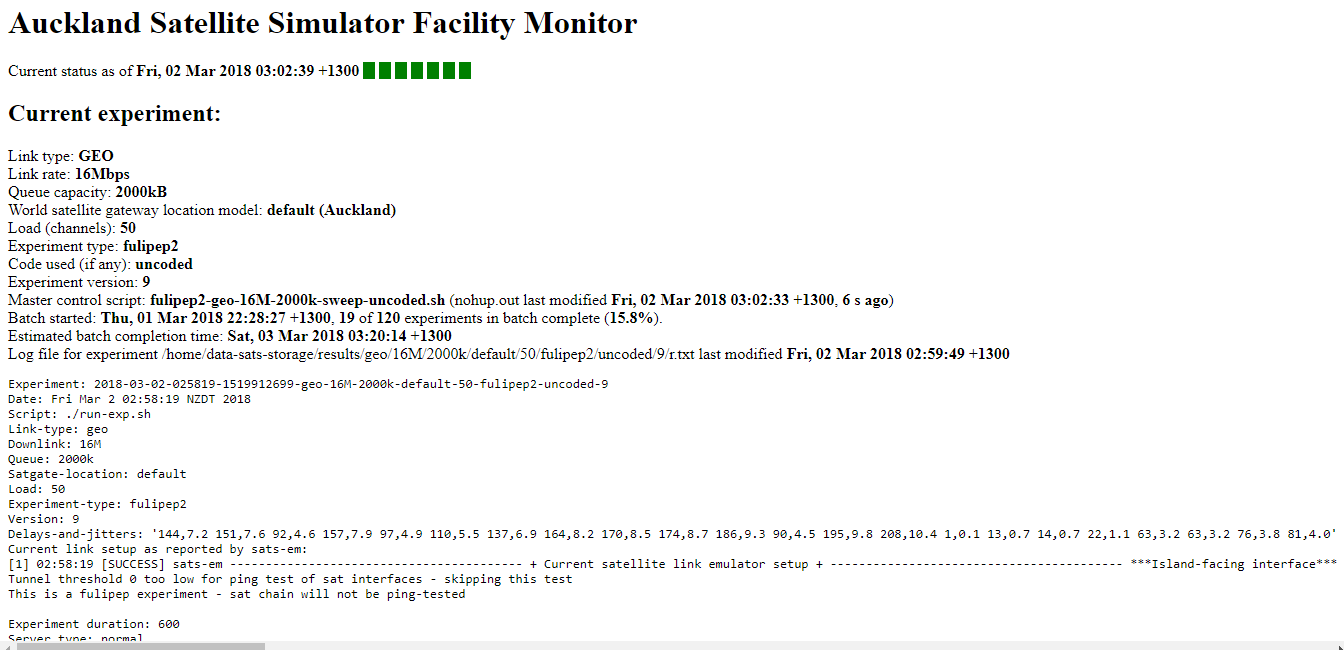
\includegraphics[width=0.87\textwidth]{experiment.PNG}
    \caption{University of Auckland Pacific Island Satellite Simulator Facility Monitor}
    \label{fig: experiment} 
\end{figure}

On top of that, we also had to deal with the following issues when preparing our PEP for the simulator.\\
\begin{enumerate}
\item Having to modify the experiment harness to be able to test it. That is: create startup scripts to start and stop the PEP on the PEP machine and remotely from the simulator's control machine. 
\item Adapting test scripts so they could accommodate the PEP, which includes changing experiment control files to create a new subtree for the log files for the PEP experiments, plus many smaller changes to analysis files.
\item Having to modify the proxy so it would forward ICMP and other non-TCP protocols directly as the simulator uses these during measurements. \\
\end{enumerate}
\todo{reword later as these are Ulrichs words}

Testing of the PEP required integration into the experiment harness of the simulator. This requirement was only possible after completion of the standard baselines and PEP experiments in late January. To do so, the PEP had to be modified to forward any non-TCP packets destined for the other side of the PEP. Some of your PEP's characteristics also required aspects of the experiment's harness quality control checks to be changed. These alterations took a couple of weeks to complete. \\

Last but not least, we had to test both for the "classic" 2000 kB satellite input queue capacity and for the 120 kB capacity we now recommend. \todo{(see \& cite https://application.isif.asia/theme/default/files/ISIFAsia\textunderscore 2016\textunderscore Grants\textunderscore TechReport\textunderscore UoA\textunderscore SimulationSatPAC.pdf, page 10/11)}
The results from each individual graph seen in the next section take about a week to complete as it runs its set of 120 experiments per graph. Only one set of experiments can be run on the simulator at any one time. The late access to the simulator plus the two-week simulator preparation and the time it takes for each set of experiments to run, left little room for major code changes and adjustments. \\

We also had the option of testing our PEP on an open source software based satellite network simulator like ns-2 or ns-3, but it would not be able to simulate the conditions of a Pacific Island satellite environment accurately. Our testbed is built specifically for the Pacific Island environment.\\

There are a few other limitations with these software simulations that we felt made its ability to simulate realistic network behaviour questionable:\\

\begin{itemize}
\item The software simulator uses an artificial timebase which limits the use of built-in network functionality.
\item Simulating many terrestrial latencies under high load is memory-consuming (because the simulator has to store all packets in flight)
\item Simulating a realistic mix of flow sizes is difficult. Many software simulations in the literature assume that it's enough to demonstrate that something gives a benefit if you load a link with a small number of long TCP flows (which are simulated as FTP most commonly, which is a sparsely used protocol these days).\\
\end{itemize}

\chapter{Second appendix}

The sockaddr\textunderscore ll structure is a device-independent physical-layer address ~cite{35}~\cite{44}.

\begin{lstlisting}
struct sockaddr_ll {
    unsigned short sll_family;   /* Always AF_PACKET */
    unsigned short sll_protocol; /* Physical-layer protocol */
    int            sll_ifindex;  /* Interface number */
    unsigned short sll_hatype;   /* ARP hardware type */
    unsigned char  sll_pkttype;  /* Packet type */
    unsigned char  sll_halen;    /* Length of address */
    unsigned char  sll_addr[8];  /* Physical-layer address */
};
\end{lstlisting}
\end{appendices}
